%!TeX encoding = UTF-8
%!TeX spellcheck = es_ES
%!TEX root=../../main.tex

\epigraph{Las normas están para cumplirlas, pero cuando se hacen por el beneficio o mejora de todos, si no, es el capricho de alguien que no está trabajando por el colectivo}{Ulises Barrera}

\begin{abstract}
Ponemos unas reglas y disponemos de ellas como una herramienta para facilitarnos el desarrollo de nuestra maqueta. ¿Que nos motiva a tener unas reglas?, ¿Son necesarias?
\end{abstract}

\section{Introducción}
Si bien la cita de Ulises Barrera se refiere a un evento deportivo, ante decisiones arbitrarias de sobre que coches pueden o no disputar una carrera, es un buena explicación de por que existen la reglas, para el beneficio del colectivo y no propio. No sin razón podemos preguntar ¿Que colectivo? si total, la maqueta es para mi mismo y para nadie más.

En el futuro, tendremos que modificar la maqueta, ya sea por mantenimiento o por que queramos ampliarla. El colectivo seremos nuestra versión futura y seguramente no nos acordemos de porque hicimos tal cosa o que cable es el que lleva la alimentación a la vía. Ya que como dice un gran filosofo:

\epigraph{Cuando hice este código solo yo y Dios sabíamos lo que hacia, ahora solo Dios lo sabe}{Comentario anonimo en internet}

Sabias palabras que medio en broma, medio en serio nos muestra la debilidad de nuestra memoria.

\section{Estado del arte}
Hoy por hoy existen muchas normas a la hora de hacer una maqueta. Prácticamente cualquier persona con un blog, canal de youtube o en un foro, expone sus normas, algunos humildemente pero otros de manera tajante. En este apartado trataremos de categorizar y recopilar las normas mas importantes que hemos encontrado.

Las categorías las organizamos según su rango de aplicación, de mas global a más especifica. Dando se la casualidad, que serán de las que menos apliquemos a menos y en caso de seguirlas mal de las que tienen más efecto a menos. Siendo estas:
\begin{itemize}
	\item \textbf{Legislativas}: Las que pone un gobierno o autoridad, que puedan afectar a nuestra maqueta. Suelen ser de seguridad y de sentido común.
	\item \textbf{Para fabricantes}: Son las normas que las asociaciones de fabricantes han puesto para que sus productos sean compatibles, alguna de ellas nos impactara en el diseño.
	\item \textbf{Para Módulos}: Son normas para hacer una maqueta de módulos intercambiables. debemos seguirlas si queremos ir a encuentros y que se pueda unir al resto.
	\item \textbf{Especificas o locales}: Estas las estableceremos para una maqueta en concreto, o si estamos en alguna asociación, las que ponga para poder hacer la maqueta entre varios socios.
\end{itemize}

\subsection{Normativas Legislativas}
El marco legal vigente nos establece una serie de normas en cuanto las actividades que se pueden realizar en según que sitios. No en todos los sitios, aun siendo de nuestra propiedad, podremos construir una maqueta de tren. En general estas normas son de seguridad, y como suele pasar con las leyes sobre seguridad, se ponen tras accidentes donde la gente ha resultado herida. 

Para una maqueta personal y pequeña (de una habitación normal) casi seguro que no haya muchas leyes que nos impacten, mas allá de las normas de convivencia. Aun conviene conocer ciertas normas que nos puedan impactar. 

Conviene conocer las normas que las autoridades locales tengan, podemos ver las siguientes:

\begin{itemize}
	\item \textbf{Reglas de Convivencia}: Básicamente, son el ruido máximo que podemos hacer y en que horas. Pero depende de como queramos "explotar" la maqueta algunas afecten más o menos.
	\item \textbf{Reglas de Construcción}: Aqui tendremos que mirar, si existe alguna ley o normativa que nos indique como debemos construir la maqueta, cuanto puede pesar. En que zonas de una casa. También en este apartado vemos los materiales que se pueden usar o no, por si resultan ser tóxicos en caso de incendio.
	\item \textbf{Reglas Eléctricas}: Puesto que vamos hacer una instalación eléctrica debemos conocer la normativa, para no sobrecargar los conductores. Seguramente simplemente con usar varios enchufes de la habitación sea suficiente.
	\item \textbf{Reglas Sanitarias}: Desde la ventilación que deba tener nuestra habitación, hasta los sanitarios que deba tener.
	\item  \textbf{Normativa de Actividades Económicas}: Si se va realizar una actividad económica en torno a la maqueta es necesario conocerlas. No es el objetivo de estos artículos desarrollar un plan de negocio, y si el lector esta planteándose montar un negocio, seguramente la parte de construcción ya la tenga más que superada.
	
\end{itemize}
Es cierto que esta lista se desarrolla no descartando ninguna para abarcar desde maquetas pequeñas a grandes como "Miniature Wünderland" pasando por el profesional que se dedica a construir maquetas o módulos para otros. Y que por ello muchas normas de esta categoría no se aplicaran, o podemos simplificarlas. También es cierto que ignorarlas (hasta el punto de hacer lo contrario) puede ser fatal.

En general, un maquetista que usa una habitación de su casa, o como mucho un anexo de la casa del pueblo. Solo tiene que preocuparse por no poner materiales peligrosos, no pasarse de peso (para que el suelo no se caiga), de que los cables de luz sean lo suficientemente grandes y de no hacer mucho(pero mucho) ruido por las noches.

Si somos un grupo con un local, deberemos tener en cuenta alguna norma más, como la sanitaria, pero en general, con un conocimiento básico y de sentido común sera suficiente. 

Estas normas alimentaran nuestra normativa de construcción y de explotación.

\subsection{Normativas Para Fabricantes}
En el mundo del modelismo ferroviario hay dos asociaciones de fabricantes, la NMRA de Estados Unidos y MOROP de Europa y que a su vez se han coordinado para que sean compatibles y referenciándose entre si.

Estas normas básicamente se establecen para poder correr material de cualquier fabricante sobre maquetas hechas con piezas de diferentes fabricantes. De tal forma podemos usar maquinas de Piko sobre vías Rocco y mezclar coches de varios fabricantes.

Estas normas se dirigen a lo siguiente:
\begin{itemize}
	\item Enganches
	\item Protocolos DCC y LCC
	\item Características eléctricas
	\item Propiedades de las escalas (dimensiones del material)
	\item Distancias de vías (galibo, curvas,...)
\end{itemize}
Para nuestras normativas, realmente solo necesitamos seguir las distancias de vías como una recomendación para ajustarnos a radios para que puedan pasar nuestro material.
\subsection{Normativas Para Módulos}
Otra forma de hacer maquetas es por modulos normalizados, esto son por partes y luego unir cada modulo para formar una maqueta más grande usando piezas de varias personas, pudiendo organizarlas de formas diferentes cada vez.

Los modulos normalizados estan pensados para realizar encuentros de maquetistas llegados de varias ciudades y montar una maqueta nueva cada vez.

\begin{figure}[h]
	\centering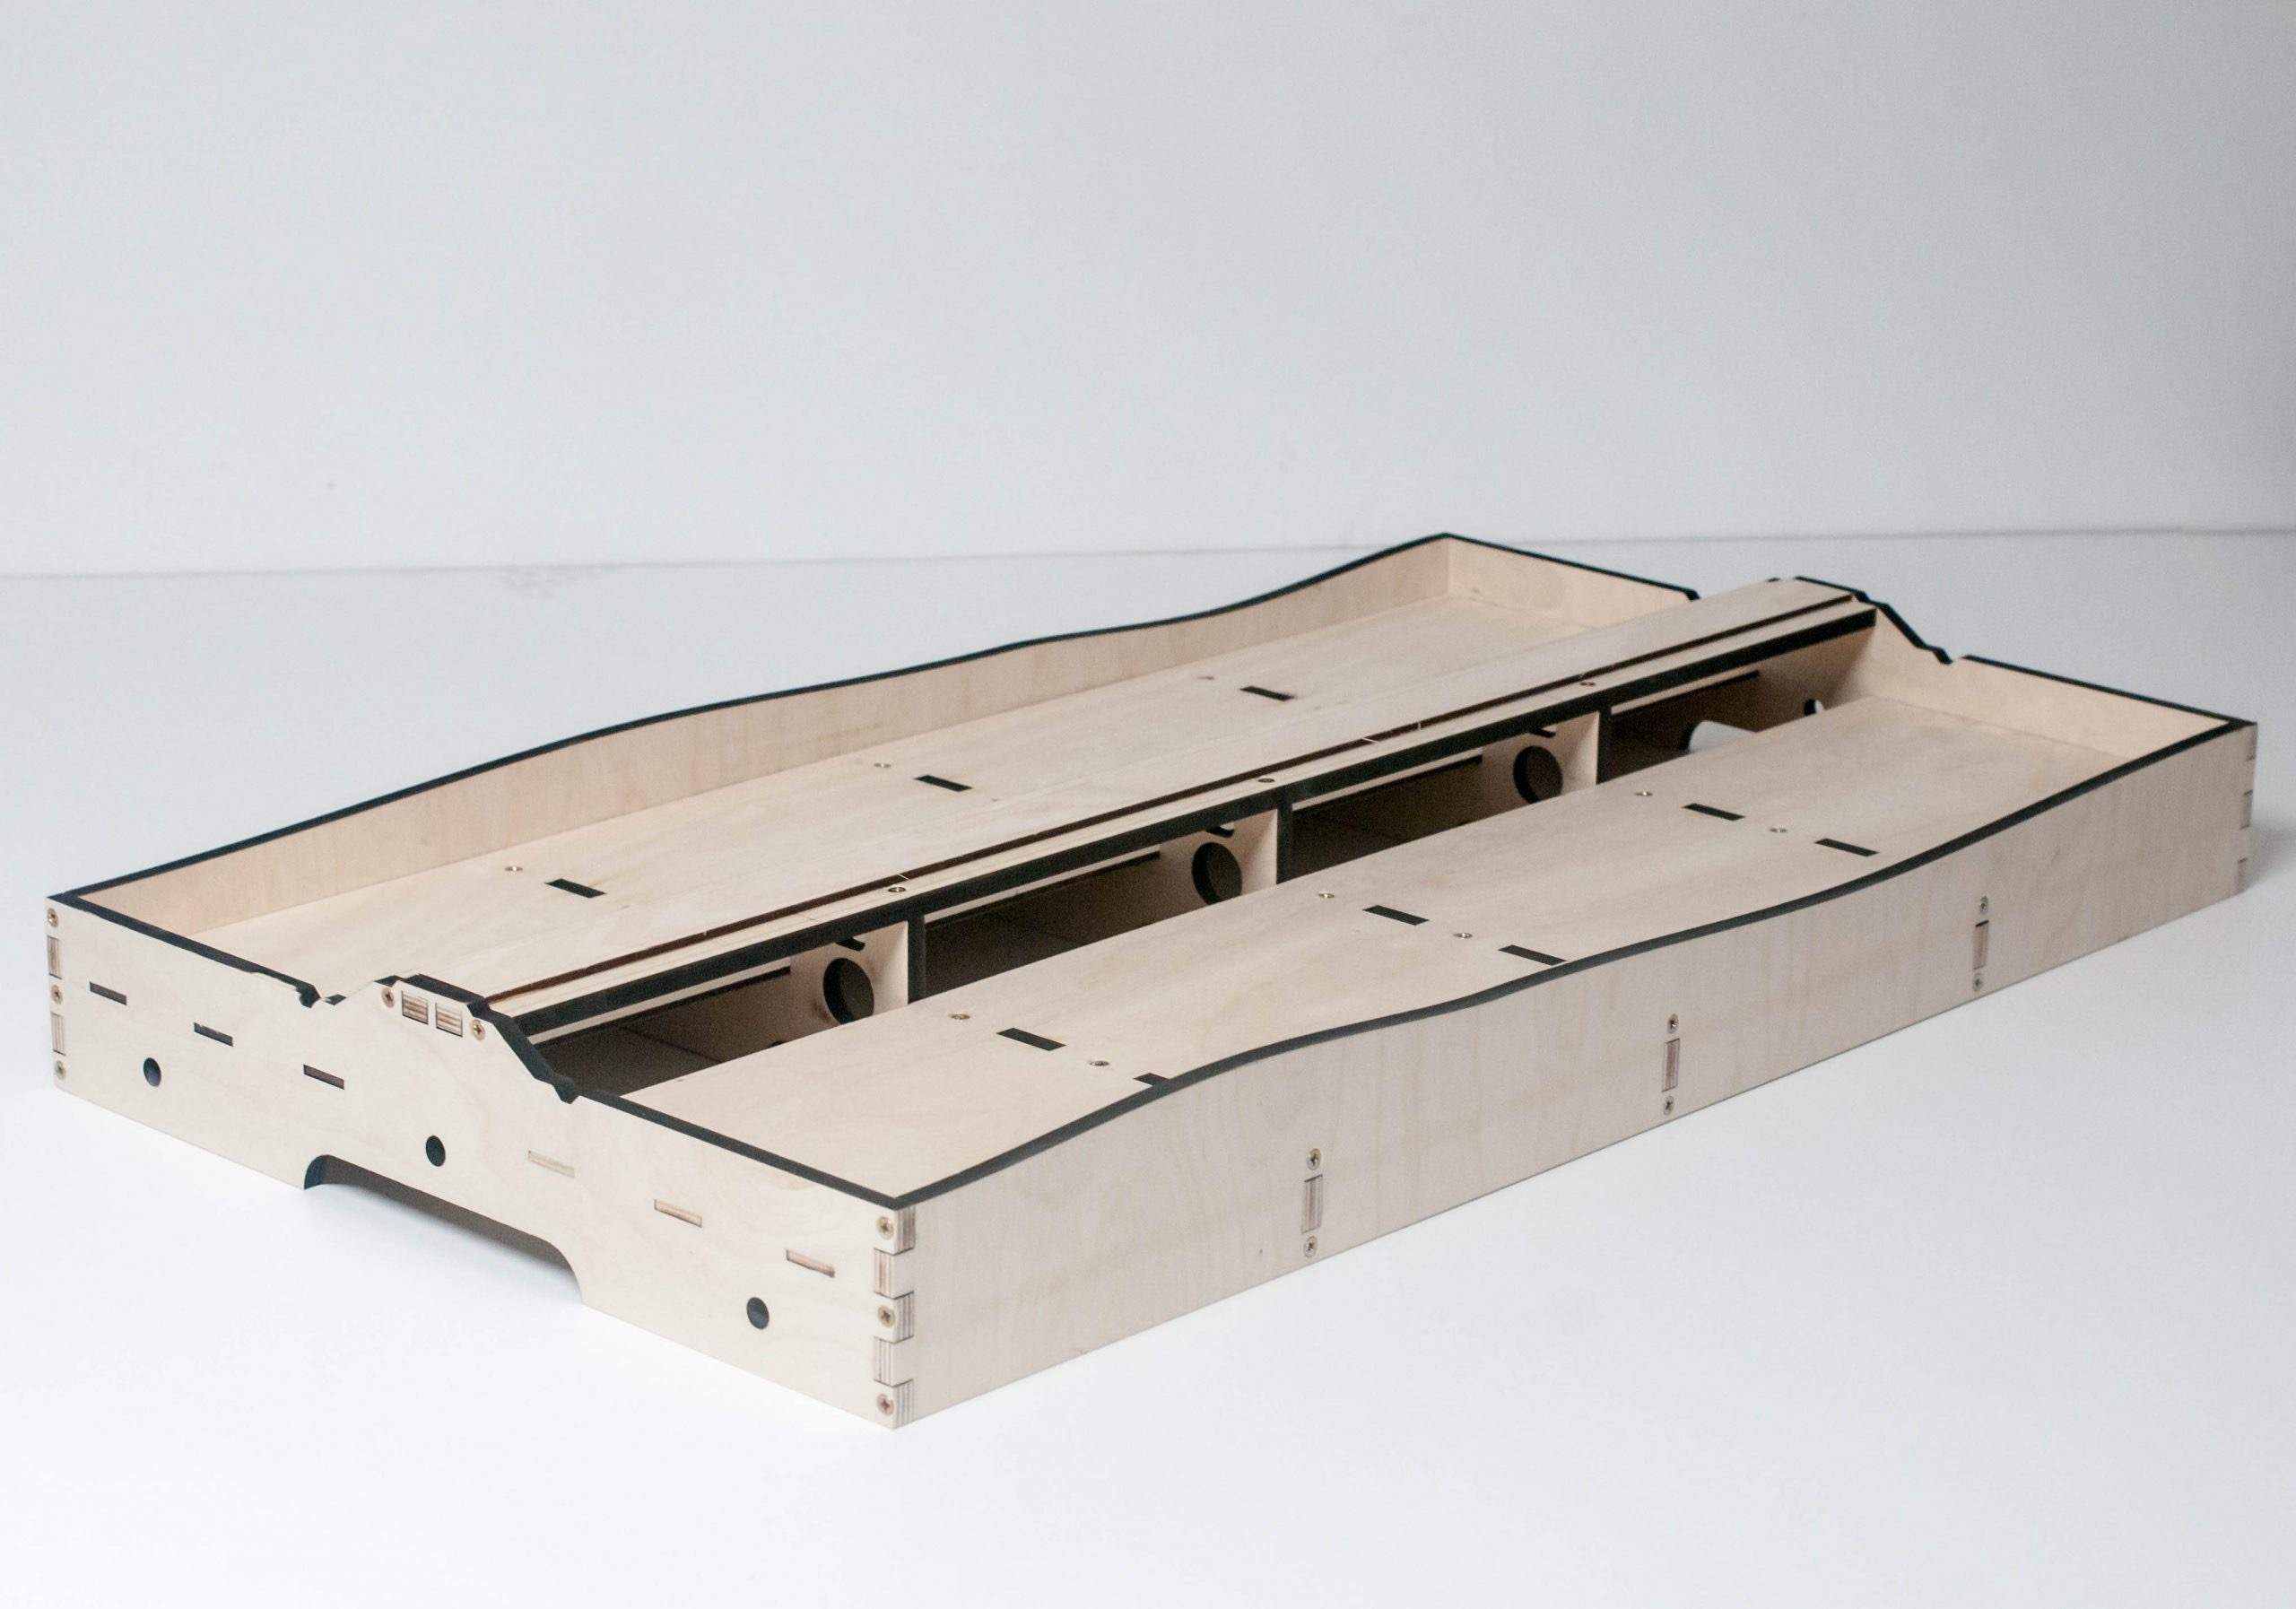
\includegraphics[scale=0.10]{chapters/0X_Normativas_01_Intro/IMG_0017.JPG}
	\caption{Modulo FreeMo TT}
	\label{fig:modulott}
\end{figure}


Es necesario tener definido una serie de cosas para que sea posible conectarlos entre si en cada encuentro y a su vez no haya modulos depentientes entre si. Estos puntos se recogen en normativas y los modulos se conocen por los nombres de dichas normativas, Modulos Maquetren, Free-Mo, T-Track,... . 

La organizacion de cada encuentro decide que normativa usar y si hay alguna varicion sobre las normas oficiales. Dicha organizacion tambien suele ser la responsable de tener modulos especiales, que  se salen de la normativa pero son necesarios, como las curvas, bucles o similares.

Como minimo las normativas modular debe definir:
\begin{itemize}
	\item \textbf{Perfil de conexion}: Esto es el perfil que debe mostar un modulo para que al menos las vias coincidan al juntar. Y asi los trenes pasar de modulo a modulo.
	\item \textbf{Conexion Mecanica}: O la forma de unir y anclar dos modulos entre si. De esta manera no se podra desplazar un modulo sin mover el otro.
	\item \textbf{Conexion Electrica}: Es decir los conectores para pasar la corriente a las vias.
\end{itemize}

\begin{figure}[h]
	\centering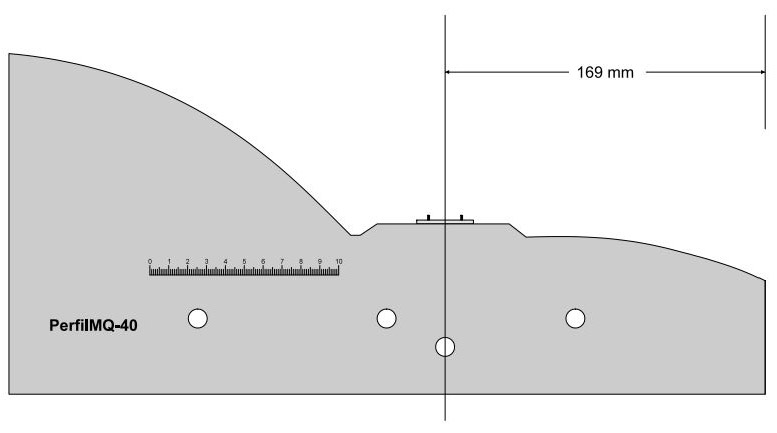
\includegraphics[scale=0.5]{chapters/0X_Normativas_01_Intro/PERFILMQ40.jpg}
	\caption{Perfil Maquetren MQ-40}
	\label{fig:perfilmq40}
\end{figure}

Pero normalmente suelen definir tambien:

\begin{itemize}
	\item \textbf{Perfil escenico}: Ya no solo el perfil sirve para que las vias coincidan, sino tambien el paisaje, de tal forma que se vea una continuidad escenica\footnote{Al menos sin saltos bruscos, pues cada modulo tendra colores diferentes}.
	\item \textbf{Altura de los modulos}: Desde el suelo.
	\item \textbf{Dimensiones}: Esto es cuanto debe medir un modulo, una dimension ya la tenemos fijada por el perfil, pero la otra puede ser más o menos libre. Fijarla a un valor permite, al encuentro, facilitar la organizacion de la maqueta y cambiar modulos de sitio a voluntad, puesto que todos miden lo mismo. Dejarla libre, dota de mayor creatividad al creador del modulo, pero la maqueta montada requerira de un esfuerzo mayor de montaje.
	\item \textbf{Forma de construir}: Hay normativas que indican como exactamente hay que crear el modulo. Suelen ser más una recomendacion que una obligacion, pero en caso de concurso puede ser razon de descalificacion. 
	\item \textbf{Conexion Electrica}: Ademas de la conexion de la via, la conexion de energia a los accesorios. Tambien en esta punto pude ser el tipo señal (DCC, Analogica,...) a las vias
	\item \textbf{Otros}: Una normativa puede ademas definir otras cosas que considere importante como puede ser el frontal, inclusion de logotipos, cartel identificador,... .

\end{itemize}

Por ultimo algunos encuentros permiten libertad en los modulos mientras se provea de algun lado normalizado para que se puede conectar a otros modulos.
Por ejemplo permiten tener un conjunto largo de modulos propios, pudiendo conectarse entre si como el maquetista quiera siempre y cuando haya al menos un lado normalizado. Como por ejemplo una estacion larga.
  
\subsection{Normativas Especificas o locales}
Por ultimo, a manera muy local, se pueden poner otras normativas que haya que cumplir en la maqueta. En esta categoria podrian entrar tanto las que se pongan para una maqueta concreta o una asocicion ponga en su maqueta de tal forma que los socios puedan hacer partes por su cuenta y luego juntarlas en el local social.

En este ultimo caso difiere de los modulos en que el objetivo es poder partir una maqueta concreta en segmentos "fijos" y hacerlo diferentes personas. Una vez montada va a ser permanente y un segmento conectara siempre con los mismos compañeros, no tienen que ser intercambiables.

\section{Motivacion de las Reglas}
Como podemos suponer las reglas se han ido creando y modificando por una u otra razon. A veces estas razones se olvidan o desaparece la necesidad, pero la regla sigue. Lo que nos lleva al refranero popular y sus maravillosas contradicciones:

\epigraph{Las reglas estan por una razon.}{Refranero popular español}

\epigraph{Las reglas estan para romperlas.}{Refranero popular español}

La primera cita nos dice que sigamos las reglas por que tienen una razon, y la seguna nos dice que nos las saltemos, una contradiccion en toda regla. El significado completo es que todas las reglas estan por una razon, si no sabes cual es siguela por si acaso, pero si la sabes y no se aplica su razon saltatela.

Es decir debemos conocer siempre las normas que se nos aplican y su motivacion, y seguirlas siempre al pie de la letra a menos que no se apliquen a nuestro caso.

En general la motivacion para cada tipo de normativa es:

\begin{itemize}
	\item \textbf{Legislativas}: La mayor parte de estas reglas estan relacionadas con la seguridad. Segun lo que queramos hacer tendremos unas u otras.  

Dentro de la creacion de maquetas lo más probable es que nos afecten legislacion para instalaciones electricas domesticas (a menos que sea muy muy grande) y referidas al peso/montaje. Seguramente podremos consultar a un electricista o un carpintero \footnote{Un amigo te cobrara en cafes, pero siempre se puede contratar a un profesional para hacer las adaptaciones pertinentes}. En caso de querer hacer algo más complicado recomendamos contratar una asesoria legal o un gabinete tecnico.  
	\item \textbf{Para fabricantes}: De estas normas nos fijaremos sobre todo en las dimensiones minimas y recomendadas que debemos seguir, como por ejemplo el radio minimo de las curvas. Si las hemos cumplido y luego no nos va bien algun tren, podemos asegurar que el problema viene de fabrica y no por nuestra maqueta.
	\item \textbf{Para Módulos}: Si queremos hacer un modulo para encuentros debemos seguirlas al pie de la letra, pero en caso de duda consultar con la organizacion. Incluso si no vamos a hacer un modulo como tal, nos conviene conocerlas puesto que son una fuente de ideas provadas para conectar varias secciones. 
	\item \textbf{Especificas o locales}: En este punto es donde debemos hacer más esfuerzo puesto que son las que nos ahorran muchos problemas en el futuro. Nos tocara hacer nuestras propias reglas y normas, sera un esfuerzo importante, pero cuando tengamos que hacer cualquier cosa, podremos ir más rapido y perder tiempo intentando averiguar como van las cosas.
\end{itemize}

\section{Resultados y Discusion} 
No hemos querido entrar en detalles de normativas especificas, para poder abarcar muchos más lectores. Puesto que en cada lugar existiran unas normas u otras. Ya bien sea por diferente legalidad o por prefencias de la zona (T-Track vs Free-Mo).

\subsection{Legislativas}
En el termino Legistalivo podemos ver las diferentes normas que existen para el cableado electrico de una casa (o de uso industrial), pero estas varian de pais a pais. Estas variaciones podemos pensar que nos afectan a lo que se ve tipo de enchufe o voltaje\footnote{Si viajamos al extranjero tenemos que llevar adaptatores y asegurarnos que nuestros dispositvos soportan 110V y 220V}
pero en la practica hay muchas normativas que cumplir, tamaño del conductor, materiales validos, distanciuas entre los elementos,... Y por suerte o por desgracia varian de pais a pais o incluso de ciudad a ciudad\footnote{Realmente de provicias, condados o como sea la organizacion territorial}.

En este aspecto de normativas legales, proponemos desde este capitulo que pensemos en tres posibles situaciones y actuemos en consecuencia.
\begin{itemize}
	\item \textbf{Maqueta Grande o Negocio}: Si vamos a montar una maqueta tamaño club, para lo cual hemos adquirdo un local o hemos decidido montar un negocio entorno a la maqueta/s. Debemos aseguranos con profesionales de que el local cumple las normativas correspondientes.

Como toda adquisicion de locales requiere una adecuacion al uso que se le va dar a dicho local, recomendamos encarecidamente aprovechar este momento para contratar a los profesionales que correspondand

Al menos se tendra que revisar que el local:
	\begin{itemize}
		\item Puede soportar el peso de la maqueta junto con otros muebles\footnote{Armarios, sillas, mesas, neveras, televisiones, ...} y de todos los visitantes
		\item Cumple con la normativa electrica para la maqueta, iluminacion,...
		\item Existen los elementos sanitarios y de seguridad correspondientes segun normativa
	\end{itemize}

	\item \textbf{Maqueta Mediana Casera o en habitacion Nueva}: En el caso que no entremos en el caso anterior, pero creamos que nuestra maqueta va a ser más pesada que un armario lleno, vamos a necestir más enchufes/circuitos de los que ya tenga la habitacion o tengamos dudas sobre la construccion de la misma. Recomendamos igualmente contratar a algun profesional. 
	\item \textbf{Maqueta Pequeña Casera en habitacion Existente}: Si vamos a montar una maqueta pequeña, de poco peso
\end{itemize}
En resumen si vamos a usar un negocio, o realizar una adaptacion grande, recomendamos encaridamente contratar a profesionales que se encargen. Pero si vamos a utilizar un lugar conocido y seguro es una sugerencia, segun la confianza que tengamos en la construcción.
\section{Conclusiones}
\section{Próximos pasos}

\section{Bibliografía}
\printbibliography[heading=subbibliography]
